\section{Who invented ConvNets and why?}

It is a little difficult to answer this question directly and clearly. There are of course multiple people who have contributed to the advancements that led to the convolutional neural networks of today. In this section we will look at a couple of important people who made the biggest contributions, and try to discover what motivated them towards the inventions.\\

\subsection{Kunihiko Fukushima}

The neural network that many consider as the root of convolutional networks was the neocognitron. Some say this was the first ConvNet \cite{sch, fuzzy}, while others call it the inspiration that led to ConvNets \cite{dl-lecun, history}. Anyhow, the neocognitron was invented in 1979 by Kunihiko Fukushima. It was first described in a Japanese paper \cite{jap} and one year later he published an English version on the same topic \cite{neocog}. Let us have a look at the man himself.\\

Fukushima, shown in \autoref{fig:fuku}, was born in 1936 \cite{about-fuku} on the island of Taiwan, which was under Japanese rule at the time. His family moved to Japan after the second world war. He became interested in electronics when an uncle gave him a disassembled electric motor to play around with. Little Kunihiko built a radio and even an electric train. This might have motivated him to study Electronics for his bachelor at Kyoto University, which he finished in 1958. Later on in 1966 he would also achieve his PhD there.\\

\begin{figure}
    \centering
    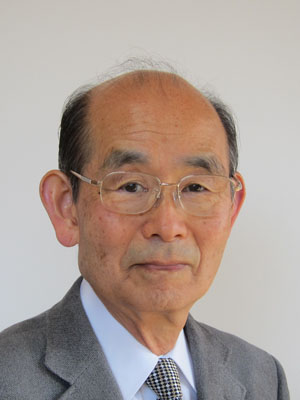
\includegraphics{images/Fukushima.jpg}
    \caption{Kunihiko Fukushima, the inventor of the neocognitron. Source: \cite{fuzzy}}
    \label{fig:fuku}
\end{figure}

During his PhD, Fukushima joined a research group on visual and auditory information processing at Japan's national broadcasting company NHK. He worked together with neurophysiologists to investigate the biological brain, which is the final destination of broadcasted signals. He was especially interested in modelling the higher brain functions, like the visual system, and applying that to an artificial neural network \cite{fuzzy}. He has received multiple awards for the neocognitron he came up with, and his further work on neural networks.  Extensions of his neocognitron are still being developed, and Fukushima himself is also still publishing. Just last year (2019) at the age of 83 he wrote about reducing the computational costs of a deep neural network \cite{83}.\\

Working together with neurophysiologists contributed to Fukushima's invention of the Neocognitron. In his paper \cite{neocog} he specifically mentions the inspiration coming from the discoveries of Hubel and Wiesel. These two men uncovered the hierarchical, layered strucuture of the visual cortex while studying the brains of cats in the early 1960's \cite{hubel, wiesel}.


\subsection{Yann LeCun}



\subsection{Other major advancements}


Weng (1993) later replaced Spatial Averaging by "Max-Pooling" (MP), which is widely used today \cite{sch}.
% eigen woorden nog

Ranzato et al. (2007) first applied BP to Max-Pooling ConvNets (MPCNNs); \cite{sch}











